\documentclass{article}
\usepackage{amsmath} % equation, align, matrix, *, &, \\, \left, \right
\usepackage{graphicx} % figure
\usepackage{subcaption} % subfigure
\usepackage{comment} % To comment
\usepackage{hyperref} % To hyperlink and ref
\usepackage{enumitem} % To list
%\usepackage[ngerman]{babel}
\usepackage[utf8]{inputenc}
\usepackage{wrapfig}
\usepackage{ulem}
\usepackage[backend=bibtex,style=numeric]{biblatex}
\usepackage{subfiles} %multifile latex projects
\usepackage{multirow}
\usepackage{booktabs}
\usepackage{color,soul}
\usepackage[table,xcdraw]{xcolor}
\usepackage{float}

%\usepackage{fontspec}
\graphicspath{{images/}{../images/}}

\bibliography{bibs} 

\title{La Caza del Tesoro}
\author{Grupo K: \\
	Tegshigzugder Otgonbayar \\
	Tim Reiprich \\
	Torres Ruiz Daniel Rafael \\
	Gómez Baco José \\
	Yepez Chavez Leticia Denise }

\begin{document}

\pagestyle{plain}
\pagenumbering{gobble} %hide page numbers

\maketitle
%\section{}
%\subsection{}
%\subsubsection{}

%\paragraph{}
%\subparagraph{}

%\paragraph*{}\mbox{}\\

\newpage

\pagenumbering{arabic} %show page numbers in arabic
\tableofcontents % from the section headings
\newpage

%\listoffigures
%\listoftables
%\newpage

%\verb||

\section{Introduction}
In the project of the course Cloud Application Development we were to develop a web application for a Treasure Hunt Game. By the given requirements we were to use different technologies of ...

\section{General description}

* deploy over a PaaS cloud \newline
* https://github.com/DRTorresRuiz/LaCazaDelTesoro

\subsection{Programming languages and frameworks}
\begin{itemize}
\item project created using the Django framwork because Python every group member knows this language and the framework is supposed to be beginner friendly
\item Python 3.7 and Django 2.2.8
\item for certain tasks like the interaction with Google Maps JavaScript had to be used as there is no explicit Python API
\item application deployed using Heroku (easy to handle, provides possibly useful add-ons)
\item Bootstrap 4.1 and Jquery 3.4.1
\item Djongo 1.2.36 to join MongoDB and Django framework
\item Django-geoposition to manage coordinates
\end{itemize}


\subsection{Treasure Hunt}

The Treasure Hunt is a competition game in which a group of participants. They must find a series of treasures scattered throughout a play area. The location of each treasure will come indicated by a clue that suggests where it is hidden. The first winner will win the game. So the main goal of the game is to locate all the treasures.

\section{Components} % Apps
The Django project is split into multiple apps. Each app handles one component of the whole project. This is done to get a clear structure of the project and to simplify parallel work. Each of the following sections will explain the functionality and implementation of one specific app.
\subsection{Registration}
\begin{itemize}
\item handles user login, storing of user data and logout
\item functionality provided by django-social-auth
\item only logout is done using the django standard logout as earlier mentioned module uses the same models
\item uses OAuth 2.0 to enable interaction with social network APIs $\to$ we used Google+ API
\item module redirects new user to Google+ Login homepage, stores known users in database and provides our homepage with needed information about the user
\item API can be configured using the Google developer console 
\item login\_required (requires user to log in to access a certain view) and user.is\_authenticated (possibility to check if user is logged in) are used in different apps of the project
\end{itemize}
\subsubsection{Homepage}
\begin{itemize}
\item contains initial view of our website
\item shows overview of current and finished games etc.
\item provides access to detail views of games and the possibility to log out
\item can only be accessed if user is logged in to a Google account, otherwise user is redirected to registration app (\@login\_required before view)
\end{itemize}
\subsection{Chat}
\begin{itemize}
\item contains functionality of interaction between users in the same game
\item add descrption how chat works and why this implementation was chosen
\item backend uses Redis to transmit the messages
\item locally a docker container providing a Redis server was used but couldn't be launched on Heroku
\item Heroku provied add-on "Heroku Redis" which was used to launch a Redis instance in the cloud to enable transmitting messages without requiring a local Redis server
\end{itemize}
\subsection{Game}
\begin{itemize}
\item provides all functionality in relation to a single game
\item the functionality developed in this section can be divided into the following:
\begin{itemize}
	\item game relationship
	\item game creation
	\item game supervision
	\item game play
	\item administration
\end{itemize}
\end{itemize}
\subsubsection{Game relationship}
\begin{itemize}
	\item provides access to aplication games
	\item allow to register in a game a play 
	\item there are three lists with games: in which the user is registered, all games and games created by the user
\end{itemize}
\subsubsection{Game creation}
\begin{itemize}
	\item all users can create games with treasures
	\item the game is created indicating the name and the play area
	\item to create a treasure the user must set a name, clue, solution coordinates and an optional image
\end{itemize}	
\subsubsection{Game supervision}
\begin{itemize}
	\item only the creator of game or administrator can see the information about the game status
	\item show treasures coordinates with markers in a map, the game status and users who have found each of the treasures
	\item the creator can reset a game, deleted all treasure findings data recorded.
\end{itemize}
\subsubsection{Game play}
\begin{itemize}
	\item the registered user can access to play game if the game are not finished
	\item the user coordinates are retrieved from the browser and in case it is not possible the user would be allowed to select the coordinates by selecting on the map
	\item the user must upload a image to prove it
	\item when a user finds all the treasures, the game ends and other users cannot find more treasures
\end{itemize}
\subsubsection{administration}
\begin{itemize}
	\item administrator users can see the status of all games
\end{itemize}
\section{Database}
Below is the diagram of the database used in the application:
\begin{figure}[H]
	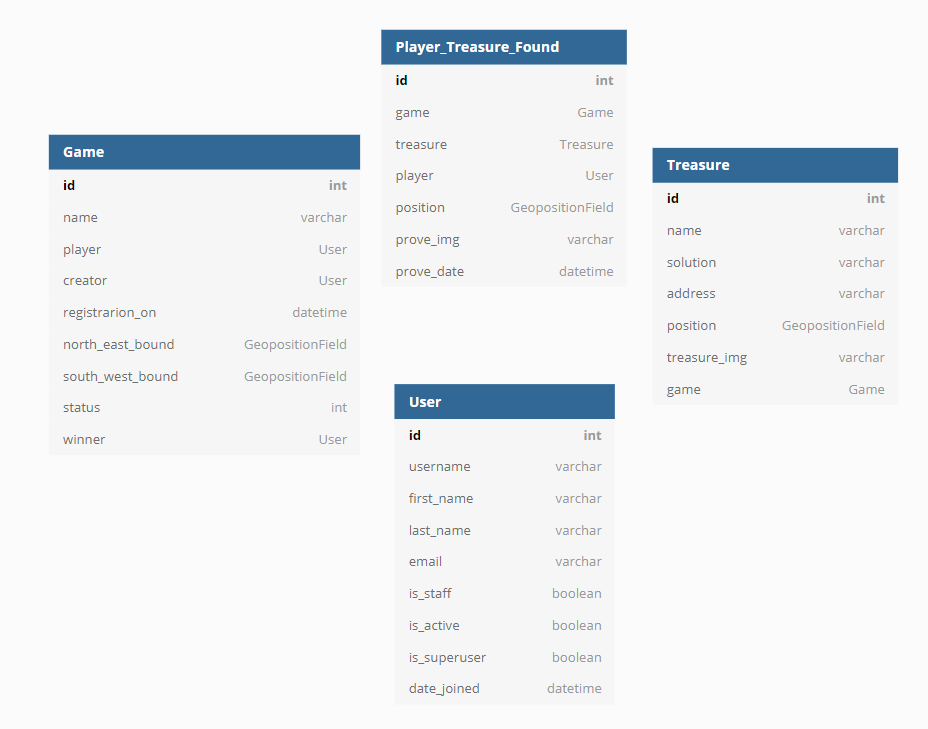
\includegraphics[width=\linewidth]{img/database.PNG}
	\caption{Database.}
	\label{fig:database1}
\end{figure}
  
We use user entity provided by Django framework and others entities that are not shown as they are typical of the framework
\section{User manual}
\begin{itemize}
\item required setup (?)
\item explanation of user interface
\end{itemize}
\newpage

\section{Limitations}
\begin{itemize}
\item limitations of our project
\item difficulties encountered
\item possible improvements in the future
\end{itemize}

\section{Summary}
Through this project we were able to

It is very interesting to study a 

\end{document}

\begin{comment}

\end{comment}
